\usetikzlibrary{calc}
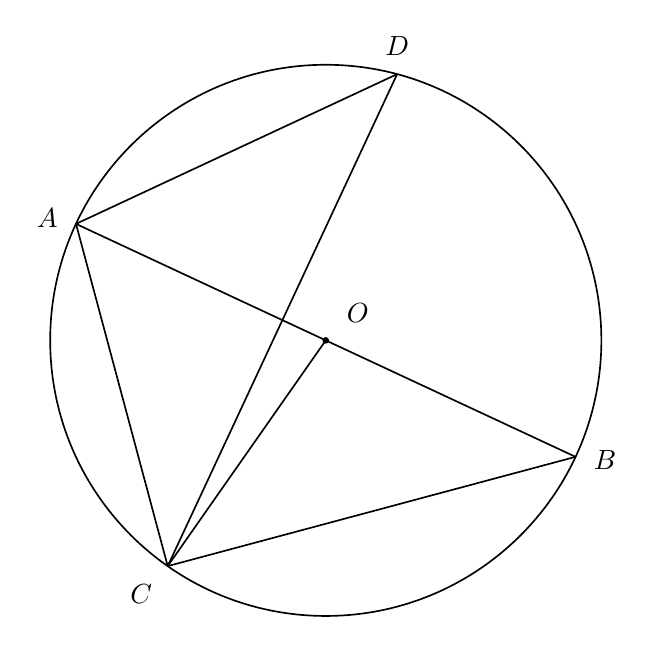
\begin{tikzpicture}[x=1cm,y=1cm,line width=.6pt,font=\normalsize]
\coordinate (O) at (0,0);
\coordinate (A) at (-3.172077,1.479164);
\coordinate (B) at (3.172077,-1.479164);
\coordinate (C) at (-2.007518,-2.867032);
\coordinate (D) at (0.905867,3.380740);
\draw[black] (O) circle[radius=3.5cm];
\draw[black] (A)--(B);
\draw[black] (A)--(C);
\draw[black] (C)--(B);
\draw[black] (A)--(D);
\draw[black] (C)--(D);
\draw[black] (O)--(C);
\fill[black] (O) circle[radius=1.2pt];
\node[left,xshift=-3pt,yshift=2pt] at (A) {$A$};
\node[right,xshift=3pt,yshift=-1pt] at (B) {$B$};
\node[below left,xshift=-2pt,yshift=-3pt] at (C) {$C$};
\node[above,yshift=3pt] at (D) {$D$};
\node[above right,xshift=4pt,yshift=3pt] at (O) {$O$};
\end{tikzpicture}
